%!TEX root = main.tex

%%%%%%%%%%% START PROJECT REPORT CONTENT HERE
\technique{Bidirectional Path Tracing}

%%%%%%%%%%%%%%% BEGIN TEASER %%%%%%%%%%%%%%%
% Teaser figure template: uses a combination of 
% a. \includegraphics with 
%      i. cropping (with the trim and clip) commands, and
%      ii. PDF page selection (with the page command) 
% and b. tikzpicture to overlay text atop the imported image. Tikz can be used to programmatically draw and/or overlay *any kind of content* (text, vector art, MATH, etc.).
%\begin{figure*}[h!]
%\label{fig:implicitPathTracingOverview}
%	\begin{center}
%		\begin{tikzpicture}
%			\node[anchor=south west,inner sep=0] at (0,0) { %
%			    	\includegraphics[width=\linewidth,page=2,trim={0cm 19.2cm 0 0},clip]{diagrams/diagram_icons.pdf} % trim = {left lower right upper}
%     			}; %
%			\node[anchor=south west] at (2.5,1.0) { \textcolor{blue}{\textit{i}} };
%			\node[anchor=south west] at (5.65,1.5) { \textcolor{blue}{\textit{ii}} };
%			\node[anchor=south west] at (10.5,2.25) { \textcolor{blue}{\textit{iii}} };
%		\end{tikzpicture}
%	\end{center}
%	\vspace{-15pt}
%	\caption*{\textbf{Implicit path tracing} traces out paths starting from the eye (\textcolor{blue}{\textit{i}}) -- scattering at surfaces in the scene (\textcolor{blue}{\textit{ii}}) -- in the blind hope that they will eventually (\textcolor{blue}{\textit{iii}}) hit a light source.}
%\end{figure*}
\vspace{-10pt}
%%%%%%%%%%%%%%%% END TEASER %%%%%%%%%%%%%%%

%%%%%%%%%%%%%%%% BEGIN FIGURE DEFINITIONS %%%%%%%%%%%%%%%
%
%%%%%%% A convenience command for our first figure
%\newcommand{\InsetFigEyeRay}{
%% Hard-code figure label
%\renewcommand{\figurename}{Step}
%%
%\setcounter{figure}{0}  % i.
%\renewcommand{\thefigure}{\textcolor{blue}{\textit{\roman{figure}}}}
%%
%\begin{wrapfigure}{r}{0.225\textwidth}
%\vspace{-2mm} % fine tuning layout
%	\begin{tikzpicture}
%		\node[anchor=south west,inner sep=0] at (0,0) { %
%		    	\includegraphics[width=0.25\textwidth,page=2,trim={14cm 12.5cm 10cm 8.65cm},clip]{diagrams/diagram_icons.pdf} % trim = {left lower right upper}
%		}; %
%		\node[anchor=south west] at (2.3,0.5) { $\x$};
%		\node[anchor=south west] at (1.3,1.0) { $-\wo$};
%		\node[anchor=south west] at (0.6,1.6) { $\xo$};
%	\end{tikzpicture}
% \caption{\label{fig:eyeRay}Rays are traced through each pixel, scattering off surfaces, in order to form paths in IPT.}
% \vspace{-2.5mm} % fine tuning layout
%\end{wrapfigure}
%}
%
%\newcommand{\InsetFigConnection}{
%% Hard-code figure label
%\renewcommand{\figurename}{Step}
%%
%\setcounter{figure}{1}  % iia.
%\renewcommand{\thefigure}{\textcolor{blue}{\textit{\roman{figure}}\,a}}
%%
%\begin{wrapfigure}{l}{0.235\textwidth}
% \vspace{-2.2mm}  % fine tuning layout
%	\begin{tikzpicture}
%		\node[anchor=south west,inner sep=0] at (0,0) { %
%		    	\includegraphics[width=0.25\textwidth,page=2,trim={26.5cm 13.7cm 1.68cm 8.65cm},clip]{diagrams/diagram_icons.pdf} % trim = {left lower right upper}
%		}; %
%		\node[anchor=south west] at (1.2,0.03) { $\x_k$};
%		\node[anchor=south west] at (0,1.63) { $\x_{k-1}$};
%		\node[anchor=south west, rotate=-32] at (0.265,1.38) {{\large\textcolor{gray}{\mbox{$\ldots$}}}};
%		\node[anchor=south west] at (2.3,1.5) { $\ws$};
%	\end{tikzpicture}
% \caption{\label{fig:connectionRay}Paths are built recursively, by shooting a ray at each path vertex, to sample the incident radiance.}
% \vspace{-2.2mm}  % fine tuning layout
%\end{wrapfigure}
%}
%
%\newcommand{\InsetFigConnectionMade}{
%% Hard-code figure label
%\renewcommand{\figurename}{Step}
%%
%\setcounter{figure}{1}  % iib.
%\renewcommand{\thefigure}{\textcolor{blue}{\textit{\roman{figure}}\,b}}
%%
%\begin{wrapfigure}{R}{0.2515\textwidth}
% \vspace{-5.5mm}  % fine tuning layout
%	\begin{tikzpicture}
%		\node[anchor=south west,inner sep=0] at (0,0) { %
%		    	\includegraphics[width=0.2515\textwidth,page=2,trim={13.7cm 4.9cm 10cm 15.0cm},clip]{diagrams/diagram_icons.pdf} % trim = {left lower right upper}
%		}; %
%		\node[anchor=south west] at (0.9,-0.10) { $\x_k$};
%		\node[anchor=south west] at (2.80,1.30) { $\x_{k+1}$};
%		\node[anchor=south west] at (1.5,1.225) { $\ws$};
%	\end{tikzpicture}
%	\vspace{-7.5mm}
%	\caption{\label{fig:surfaceConnection}We build paths by incrementally sampling vertices.}
% \vspace{-4.2mm}  % fine tuning layout
%\end{wrapfigure}
%}
%
%\newcommand{\InsetFigPathTermination}{
%% Hard-code figure label
%\renewcommand{\figurename}{Step}
%%
%\setcounter{figure}{2}  % iii.
%\renewcommand{\thefigure}{\textcolor{blue}{\textit{\roman{figure}}}}
%%
%\begin{wrapfigure}{L}{0.235\textwidth}
% \vspace{-4.3mm}  % fine tuning layout
%	\begin{tikzpicture}
%		\node[anchor=south west,inner sep=0] at (0,2.4) { %
%		    	\includegraphics[width=0.25\textwidth,page=2,trim={26.8cm 4.9cm 0.0cm 17.75cm},clip]{diagrams/diagram_icons.pdf} % trim = {left lower right upper}
%		}; %
%		\node[anchor=south west,inner sep=0] at (0,0) { %
%		    	\includegraphics[width=0.25\textwidth,page=2,trim={0.35cm 0.40cm 26.5cm 20.6cm},clip]{diagrams/diagram_icons.pdf} % trim = {left lower right upper}
%		}; %
%	\end{tikzpicture}
% \vspace{-6.0mm}
% \caption{\label{fig:pathTermination}In IPT, paths are only terminated once they escape the scene (top) or hit a light source (bottom).}
% \vspace{-3.2mm}  % fine tuning layout
%\end{wrapfigure}
%}
%
%
%\newcommand{\ConvergenceFigure}{
%% Hard-code figure label
%\renewcommand{\figurename}{Convergence}
%% Example of an index-less figure
%%
%\renewcommand{\thefigure}{}
%\setcounter{figure}{0}
%%
%\begin{figure*}[b!]
%\centering
%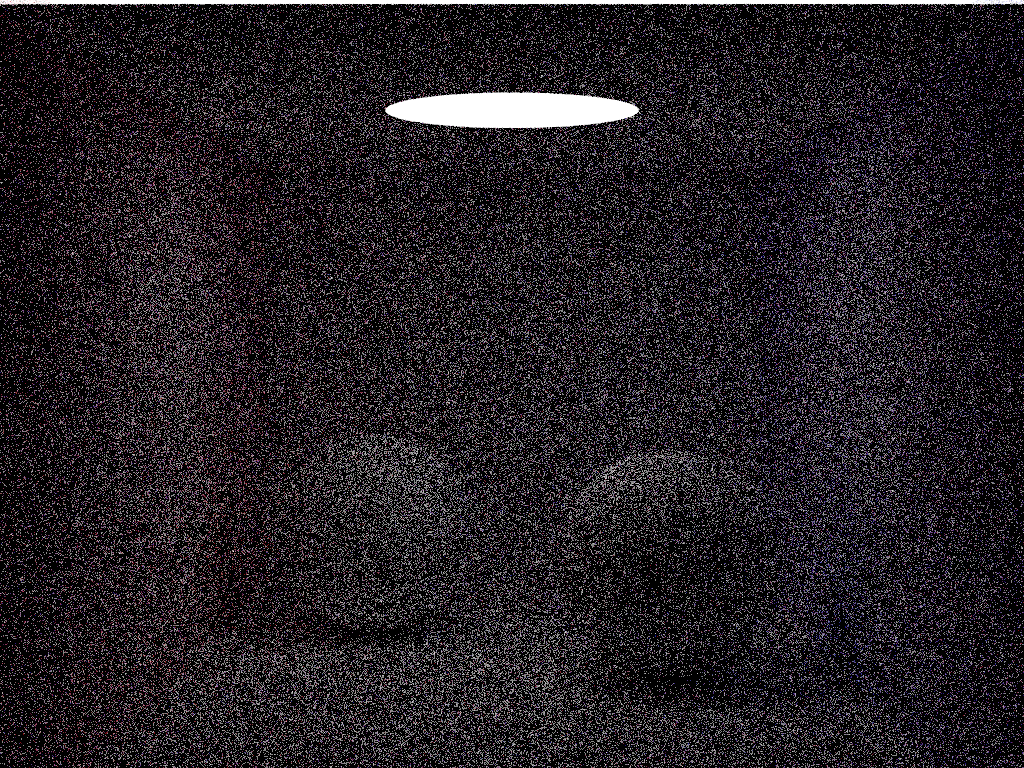
\includegraphics[width=0.245\linewidth]{images/image_4spp.png}
%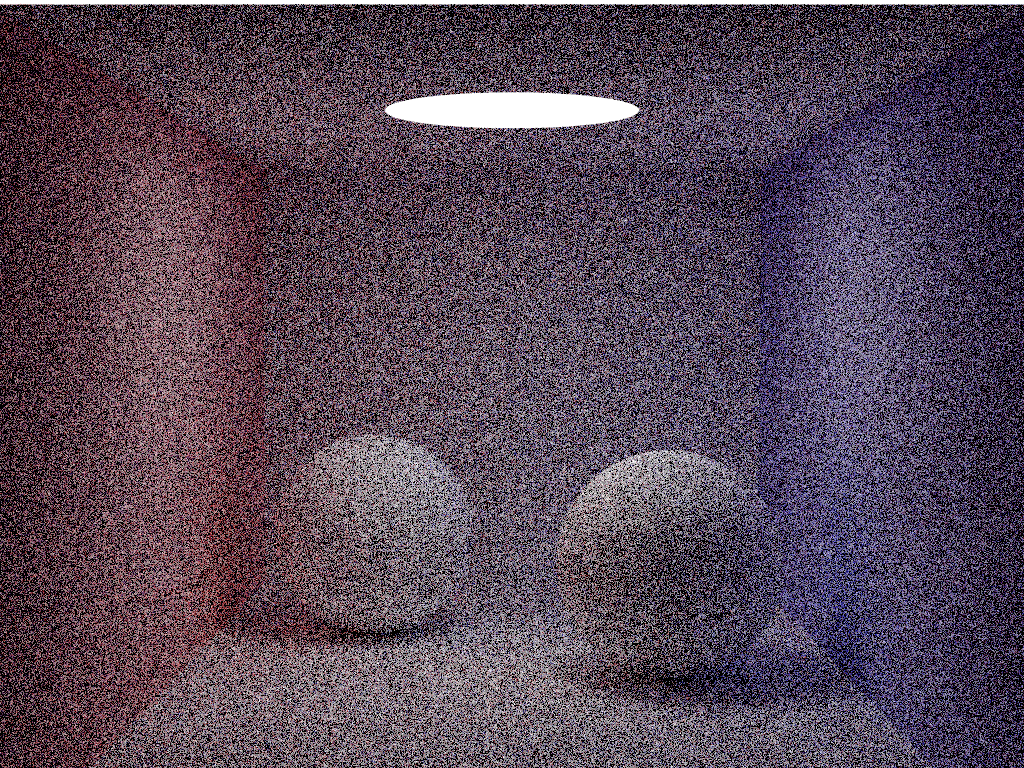
\includegraphics[width=0.245\linewidth]{images/image_16spp.png}
%%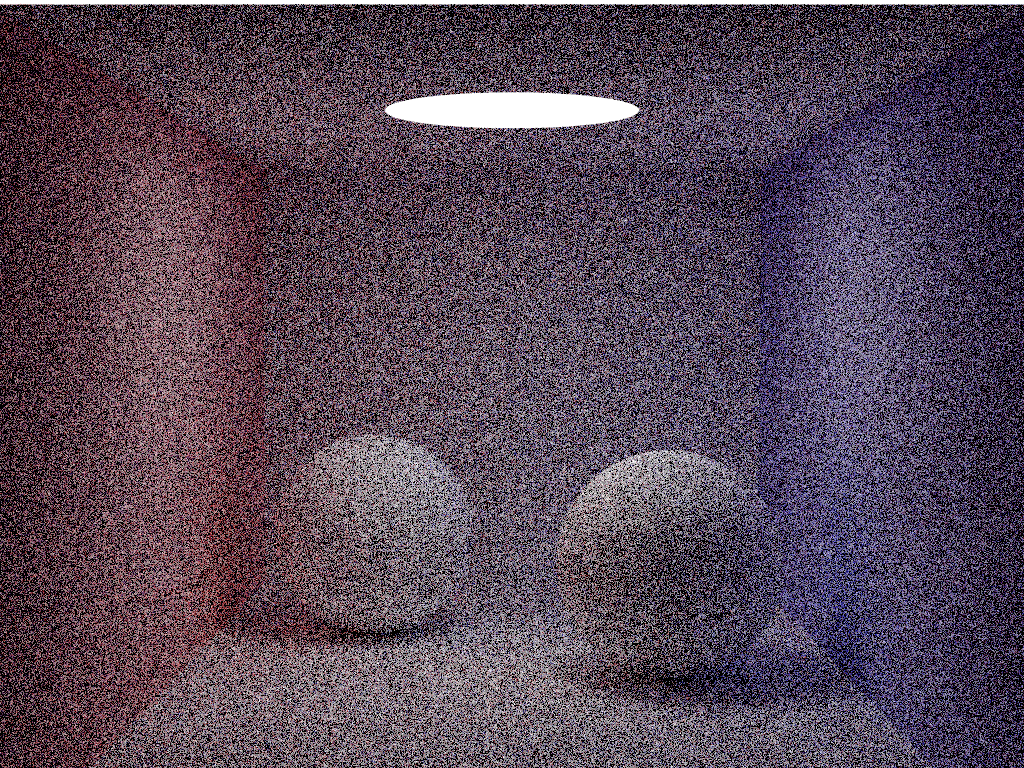
\includegraphics[width=0.166\linewidth]{images/image_32spp.png}
%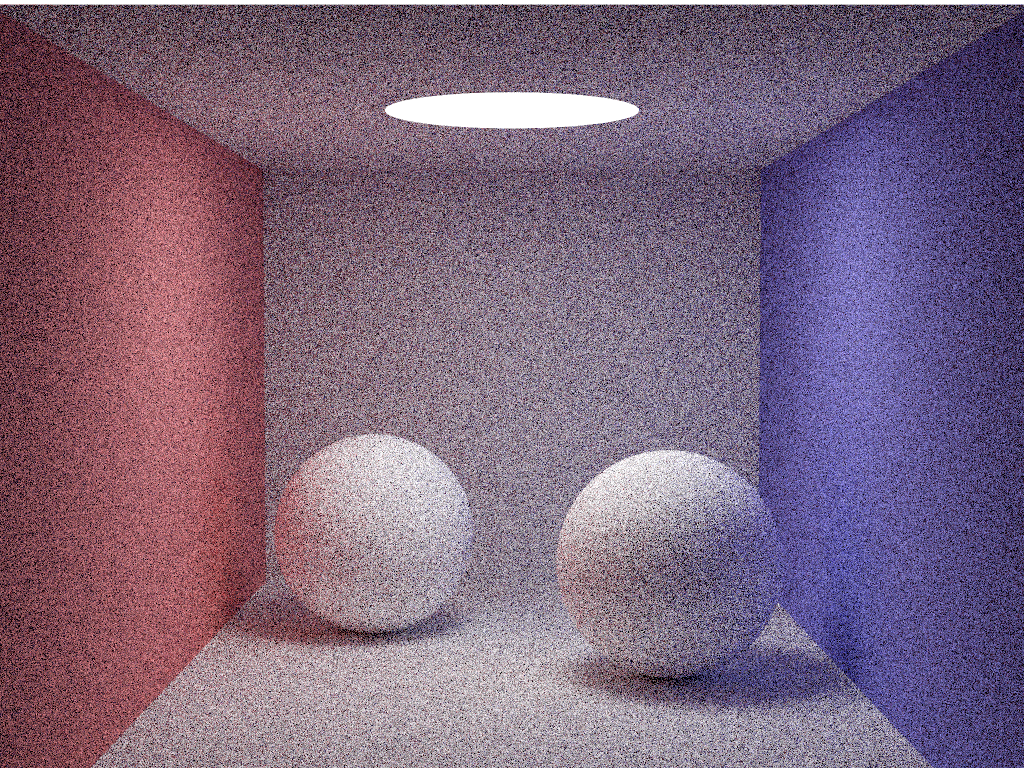
\includegraphics[width=0.245\linewidth]{images/image_64spp.png}
%%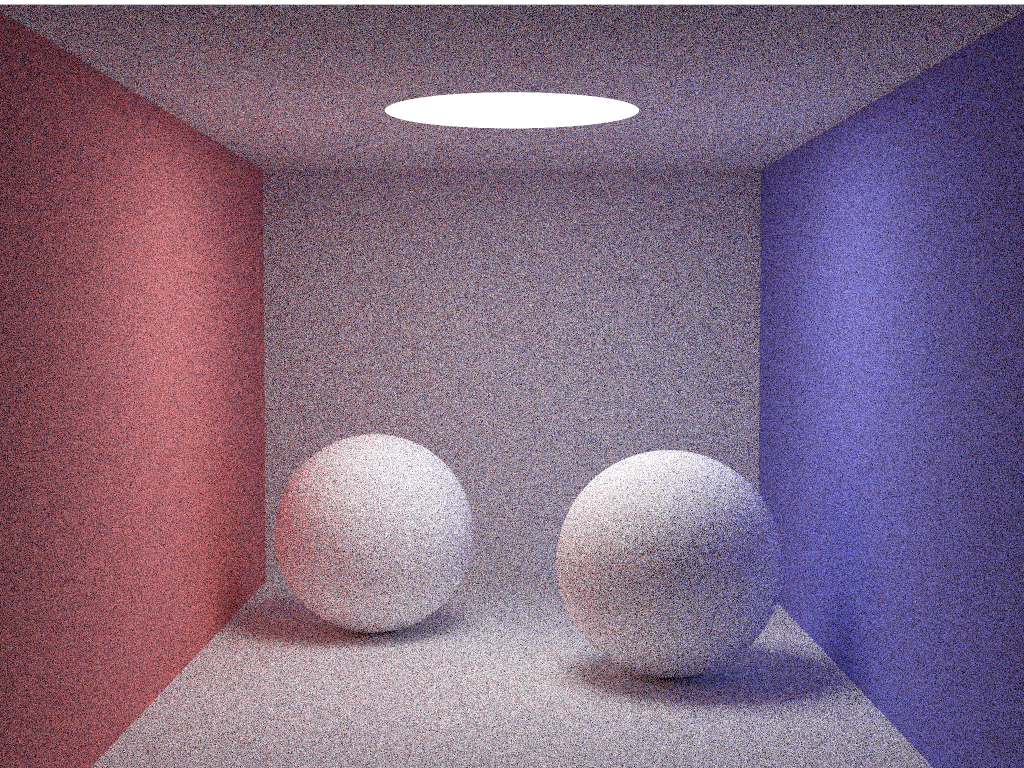
\includegraphics[width=0.166\linewidth]{images/image_128spp.png}
%%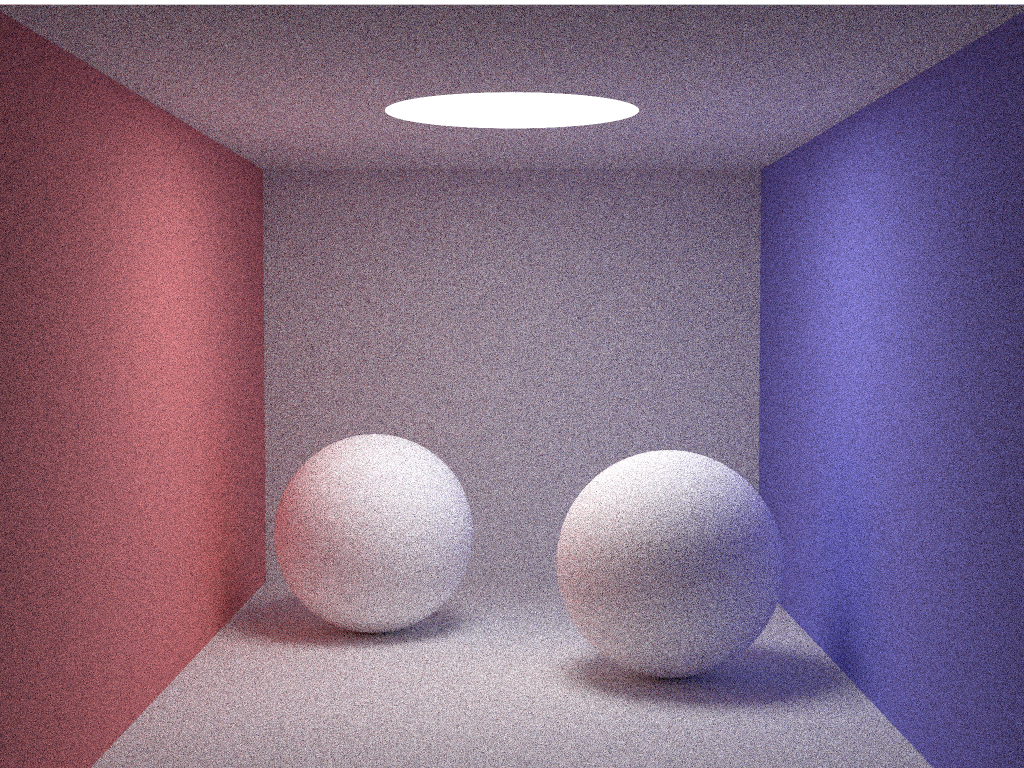
\includegraphics[width=0.166\linewidth]{images/image_256spp.png}
%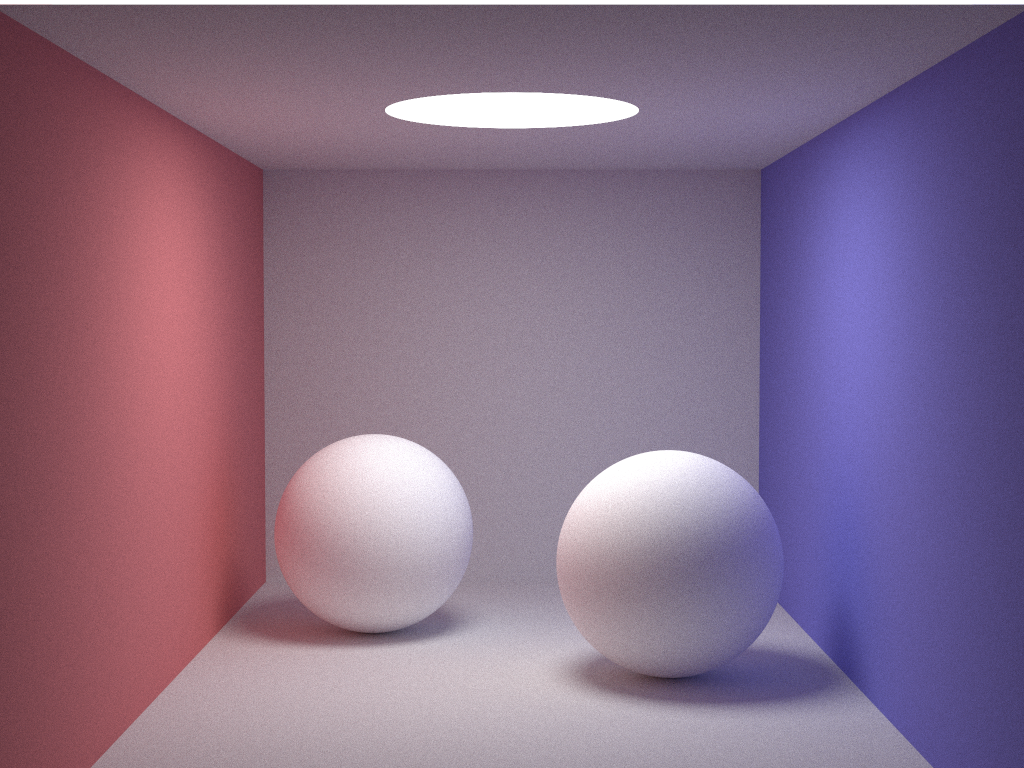
\includegraphics[width=0.245\linewidth]{images/image_4096spp.png}
% \vspace{-6.5mm} % fine tuning layout
% \caption{\label{fig:convergence}As we increase the MC sample rate, variance decreases and IPT convergences to the correct solution.}
%\end{figure*}
%}
%
%\newcommand{\CodeDiagramFigure}{
%  \vspace{0.20cm}
%  \adjustbox{valign=t}{
%	\begin{tikzpicture}
%		\node[anchor=south west,inner sep=0] at (0,0) { %
%		    	\includegraphics[width=0.495\textwidth,page=2,trim={1.8cm 8.35cm 24.2cm 9.5cm},clip]{diagrams/diagram_icons.pdf} % trim = {left lower right upper}
%		}; %
%		\node[anchor=south west] at (1.8,3.2) { \code{wo}};
%		\node[anchor=south west] at (2.80,1.85) { \code{pt.x}};
%		\node[anchor=south west] at (5.2,3.2) { \code{wi}};
%		\node[anchor=south west] at (0.5,4.825) {\footnotesize{[\textcolor{myred}{\textbf{line 9}}]}};
%		\node[anchor=south west] at (4.76,5.2) {\footnotesize{[\textcolor{myred}{\textbf{line 20}}]}};
%		\node[anchor=south west] at (5.96,3.5) {\footnotesize{[\textcolor{myred}{\textbf{line 23}}]}};
%	\end{tikzpicture}
%  }
%}

%%%%%%%%%%%%%%% END FIGURE DEFINITIONS %%%%%%%%%%%%%%%

%%%%%%%%%%%%% BEGIN OVERVIEW %%%%%%%%%%%%%%%



\paragraph{Overview}
%

\vspace{4mm}

 Light transport in scenes where only a small subset of emitters contribute energy to the image sensor, and only after undergoing many scattering events, are particularly challenging to simulate using unidirectional path tracing techniques such as implicit and explicit path tracing. For example, in a setting such as in Figure 1, only implicit paths with a second-to-last vertex on a small area on the ceiling will be able to find illumination from the light. 
%
\newline
%
Bidirectional path-tracing (BDPT) is a generalization of the standard path-tracing algorithm that can be handle indirect lighting problems far more efficiently and robustly. For each pixel of the output image, BDPT incrementally generates paths from both light sources and eye point and then combines each pair of vertices along the \textit{light subpaths} and \textit{eye subpaths}. If the \textit{connecting edge} between the pair of connected vertices is visible, the contribution of such complete light transport will be added to the radiance estimate. This note assumes a naïve connection strategy by only connecting pairs of vertices through a single pixel, although other connection strategies can have better performance.
%
\newline
%
Each connection can correspond to a separate sampling technique. The  reason that these techniques are useful is that they correspond to different density functions $p_{s,t}$ on the space of paths. All of these density functions are good candidates for importance sampling, because they take into account different factors of the measurement contribution function $f_{j}$. In practical terms, this means that each
technique can efficiently sample a different set of lighting effects.
%
\newline
%
The following estimate is computed for each measurement $I_{j}$:
%
\begin{align}
\label{eqn:measurementEquation}
F = \sum_{s\geq0}\sum_{t\geq0}p_{s,t}(\bar{x}_{s,t}) \dfrac{f_{j}(\bar{x}_{s,t})}{p_{s,t}(\bar{x}_{s,t})}
\end{align}
	
%%%%%%%%%%%%%% END OVERVIEW %%%%%%%%%%%%%%%
%	
	

%\paragraph{Overview}
%%
%Implicit path tracing (IPT) is the simplest algorithm capable of accurately computing global illumination effects in a virtual scene. This note assumes \textit{surface-only} transport (i.e., no participating media) and fully opaque objects (i.e., no transmission or refraction -- all scattering is due to reflection), although the algorithm can be generalized to handle a variety of effects.
%%
%\newline
%%
%IPT is a ``forward'' ray-tracing technique\footnote{Some sources use the term ``backward'' ray-tracing in this context, since light flows \textit{from} lights \textit{to} the eye in reality.}, meaning that paths are traced starting \textbf{from the eye}, with the hope of eventually hitting a light, and thus forming a \textit{full light transport path}. The final image is generated by averaging the contribution of many such paths, through each pixel. The main drawback of IPT is that it forms light transport paths somewhat blindly, in the sense that a (potentially long, unfinished) path can eventually end without ever hitting a light source (e.g., \textcolor{gray}{gray} dotted arrow in the \hyperref[fig:implicitPathTracingOverview]{overview figure}).
%%
%\newline
%%
%The IPT algorithm is a Monte Carlo (MC) estimator of the rendering equation~\cite{Kajiya:1986}
%%
%\begin{align}
%\label{eqn:renderingEquation}
%L(\x, \mathbf{\omega}_o) = L_e(\x, \mathbf{\omega}_o) + \int_{\Omega_{\n}} \!\!\!\! L(\x', -\wi) \, f_r(\x, \wi, \wo) \, (\n \cdot \wi) \, \d\wi \,,
%\end{align}
%where $L(\x, \mathbf{\omega}_o)$ is the outgoing radiance at a surface point $\x$ with normal $\n$ (e.g., the closest visible point from a pixel) in the direction $\wo$ towards the viewer. The outgoing radiance is the sum of the emitted radiance $L_e$ at $\x$ and the \textbf{reflected radiance}: an integral, over all incident lighting directions ${\Omega_{\n}}$ in the upper hemisphere around $\x$, of the product of incident radiance $L(\x', -\wi)$ from the point $\x' = \code{ray(}\x,\wi\code{)}$ nearest to $\x$ in the direction $\wi$, the \textit{bidirectional reflectance distribution function} (BRDF) $f_r$ at $\x$, and a cosine foreshortening factor.
%%%%%%%%%%%%%% END OVERVIEW %%%%%%%%%%%%%%%
%

%%%%I%%%%%%%%% BEGIN BASIC IDEA %%%%%%%%%%%%%%
\paragraph{Basic Idea}
%
At each pixel, the IPT algorithm averages the value of many 1-sample Monte Carlo integral estimates $\mathtt{E}^{\mbox{\tiny{1spp}}}_{\mbox{\tiny{$\Omega$}}}$ of Equation~\ref{eqn:renderingEquation} :
%
\begin{align}
\label{eqn:MCEstimateSolidAngle}
\mathtt{E}^{\mbox{\tiny{1spp}}}_{\mbox{\tiny{$\Omega$}}} \left[ L(\x, \mathbf{\omega}_o) \right] = L_e(\x, \mathbf{\omega}_o) + L(\x', -\ws) \, f_r(\x, \ws, \wo) \, (\n \cdot \ws)\big/pdf(\ws),
\end{align}
%
where, here, each 1-sample estimate forms a light path by tracing rays through the scene, evaluating the terms in Equations~\ref{eqn:renderingEquation} and \ref{eqn:MCEstimateSolidAngle} along the way (see \hyperref[sec:IPTalgorithm]{Algorithm Details} below.) In Equation~\ref{eqn:MCEstimateSolidAngle} we sample a \textbf{direction} $\ws \sim pdf(\omega)$ from a valid sampling probability distribution function $pdf$ over the solid angle measure. We form a full path by recursively evaluating the incident radiance $L(\x', -\ws)$. Note that, while Equation~\ref{eqn:MCEstimateSolidAngle} uses the \textit{solid angle form} of the rendering equation (as written in Equation~\ref{eqn:renderingEquation}), we could just as easily have used a \textit{surface area form}; in doing so, the integration domain in Equation~\ref{eqn:renderingEquation} would become the set of all scene surfaces $\mathcal{M}$ and the corresponding 1-sample MC integral estimator $\mathtt{E}^{\mbox{\tiny{1spp}}}_{\mbox{\tiny{$\mathcal{M}$}}}$ would sample \textbf{surface points} in the scene:
%
\begin{align}
\label{eqn:MCEstimateSurfaceArea}
\mathtt{E}^{\mbox{\tiny{1spp}}}_{\mbox{\tiny{$\mathcal{M}$}}} \left[ L(\x \rightarrow \xo) \right] = L_e(\x \rightarrow \xo) + L(\x \leftarrow \xs) \, f_r(\xs \rightarrow \x \rightarrow \xo) \, G( \x , \xs) \Large/ pdf(\xs),
\end{align}
%
where arrows denote directional relationships between points, the $pdf$ is one for choosing \textit{points on scene surfaces}, and the geometry term $G( \x , \xs) = (\cos\n_\x \, \cos\n_{\xs}) / |\x - \xs|^2$ includes the original cosine foreshortening factor and an \textit{additional} cosine foreshortening about the normal of the ``emitting'' surface point (and the squared-distance between the two points; see Step~\ref{fig:surfaceConnection}). These additional terms are due to the Jacobian mapping between differential solid angles (i.e., when integrating over incident directions $\Omega_{\n}$) and differential surface elements (i.e., when integrating over scene surfaces $\mathcal{M}$). Specifically, by substituting $\d\wi = G( \x , \xi) \, \d\xi / \cos\n_\x$ into Equation~\ref{eqn:renderingEquation} we can arrive at the surface-area form where the reflected radiance is an integral over $\mathcal{M}$ instead of $\Omega_{\n}$: $L(\x \shortrightarrow \xo) =  L_e(\x \shortrightarrow \xo) + \int_{\mathcal{M}} L(\x \shortleftarrow \xi) \, f_r(\xi \shortrightarrow \x \shortrightarrow \xo) \, G( \x , \xi) \, \d\xi$.
%
\newline
%
Perhaps the most important concept in IPT is that of a \textit{light transport \textbf{path}} and, specifically, one beginning at the eye and ending at the light. Both Equations~\ref{eqn:MCEstimateSolidAngle} and \ref{eqn:MCEstimateSurfaceArea} naturally lead to the formation of such paths due to the \textbf{recursive} incident radiance term $L(\x', -\wi) \equiv L(\x \leftarrow \xi)$; we (recursively) apply an MC estimator to evaluate this term since the \textit{incident} radiance at $\x$ from direction $\wi$ (or, equivalently, from surface point $\xi$) is equal to the \textit{outgoing} radiance at $\xi$ back towards $\x$. In doing so, we can arrive at the \textit{path space formulation} of the rendering equation as
%
\begin{align}
\label{eqn:renderingEquationPathSpace}
L(\x_0 \leftarrow \x_1) \!= \!\int_{\mathcal{P}} \!\! W_e(\x_0, \x_1) \, L_e(\x_k \rightarrow \x_{k-1}) \underbrace{G(\x_{0} , \x_{1}) \prod_{j=1}^{k-1} f_r(\x_{j+1} \rightarrow \x_{j} \rightarrow \x_{j-1}) \, G(\x_j , \x_{j+1})}_{T(\overline{\x})} \d\overline{\x}\,,
\end{align}
%
where $\mathcal{P}$ is the space of \textbf{all} light paths $\overline{\x} = \{\x_0 \ldots \x_k\}$, $W_e$ models the sensor's importance response\footnote{Not to be confused with \textit{importance sampling}, \textit{importance} is the radiometric dual of \textit{radiance}.}, only those paths that ``end'' at a vertex $\x_k$ on a light contribute non-zero radiance to $\x_0$, and $\d\overline{\x} = \prod_{i=0}^k \d\x_i$. The path's \textbf{throughput} $T(\overline{\x})$ combines evaluations of the geometry and BRDF terms at each path vertex. We can write a 1-sample MC estimator of Equation~\ref{eqn:renderingEquationPathSpace} as: 
%
\begin{align}
\label{eqn:MCEstimatePathSpace}
\mathtt{E}^{\mbox{\tiny{1spp}}}_{\mbox{\tiny{$\mathcal{P}$}}} = L_e(\overline{\x}_{s,k} \rightarrow \overline{\x}_{s,k-1}) \, T(\overline{\x}_s) \big/ pdf(\overline{\x}_s)\,,
\end{align}
with a $pdf$ over the distribution of light paths.\\

%\remarks{
%In \hyperref[sec:IPTalgorithm]{Algorithm Details} we present the IPT algorithm in the form of a solution to Equation~\ref{eqn:MCEstimateSolidAngle}, but it is important to understand that both the solid angle and surface area formulations can be generalized into the path space formulation. Indeed, one can readily form a $pdf$ over paths by combining (i.e., even during the process of path construction) the product of $pdf$s over surface points and $pdf$s over directions, as long as the proper care is taken to incorporate the (resp. inverse) Jacobian that maps $\d\wi$ to (resp. from) $\d\xi$.}

\vspace{-10pt} % typesetting: removing oversized whitespace
%%%%%%%%%%%%% END BASIC IDEA %%%%%%%%%%%%%%%


%%%%%%%%%%%%% BEGIN ALGORITHM DETAILS %%%%%%%%%%%%%%
\paragraph{Algorithm Details}
\label{sec:IPTalgorithm}
As with most rendering algorithms, IPT relies on the ability to query the geometry of a scene. For the purposes of our implementation, we will assume that a ray tracer is used here, where rays are traced to compute (nearest-surface) object intersections.
%
%\InsetFigEyeRay 
%
To begin, we assume that camera rays are generated and traced through each pixel. For each of these rays, the core IPT algorithm evaluates a 1-sample MC estimate of the rendering equation (i.e., Equation~\ref{eqn:MCEstimateSolidAngle}) at the nearest surface point $\x$ intersected by the ray and, ideally, the average of many such estimates is used to compute the final image. As such, IPT is trivially parallelizable over both pixels and samples (i.e., paths), and one can easily incorporate distribution effects such as pixel anti-aliasing, depth of field, or motion blur by simply assigning different spatial, lenticular, or time coordinates to each camera ray traced through a single pixel. The \code{\textcolor{myred}{Lo}} function in our code listing implements the 1-sample MC estimate in Equation~\ref{eqn:MCEstimateSolidAngle}.

%
\pagebreak % HACK: force page break for wrapfig layout purposes
%
%\InsetFigConnection
%
\noindent At each (non-emissive\footnote{We assume that luminaires do not reflect light and vice-versa (i.e., that reflective surfaces have no emission).}) surface interaction, the IPT algorithm \textit{incrementally} forms a path and accumulates an MC estimate of its throughput $T$. In the solid angle formulation, first an ``outgoing'' ray (with direction $\ws \sim pdf(\omega)$) evaluates the incident radiance $L(\x',-\ws)$ at the current vertex $\x_k$, where $\x' = \x_{k+1} = \code{ray(}\x_k,\ws\code{)}$ is the surface point nearest to $\x_k$ in direction $\ws$. We then multiply the accumulated throughput $T(\overline{\x})$ by the cosine-weighted BRDF at $\x_k$ and divide by $pdf(\ws)$ to form our estimate. We repeat the process recursively at the next vertex. Concretely, in the solid angle formulation, we multiplicatively accumulate
%
\begin{align}
f_r \Big( \x_k, \ws, (\x_{k-1} - \x_k) / |(\x_{k-1} - \x_k)| \Big)  (\n_{\x_k} \cdot \ws) \Big/ pdf(\ws)
\end{align}
%
until path termination (see below). The choice of sampling distribution $pdf$ influences the variance of our estimator but, with a valid\footnote{A $pdf$ is valid if it is non-zero in all regions of the domain where the integrand is non-zero.} $pdf$, the estimator remains unbiased. Our implementation uses a cosine distribution about the normal, $pdf(\omega) = (\n \cdot \omega) / \pi$ (implemented as \code{\textcolor{myred}{sampleCosine}} in the \hyperref[lst:IPTpseudocode]{code listing}). To draw samples according to this $pdf$, we rotate random cosine-distributed directions $\widehat{\omega} = (\theta_s,\phi_s) = (\arccos({\sqrt{\epsilon_0}}), 2\pi\epsilon_1)$ about the $z$-axis to align about $\n$, obtaining $\ws$, where $\epsilon_0$ and $\epsilon_1$ are uniform random numbers in $[0,1)$.
%
\newline
%
%\InsetFigConnectionMade 

\vspace{-13pt}
\noindent For completeness, using the surface area formulation and \textit{explicitly} sampling $\x_{k+1}$ according to a $pdf$ over surfaces (instead of \textit{implicitly} sampling it as a function of $\ws$, $\code{ray(}\x_k,\ws\code{)}$), we would accumulate the geometry-weighted BRDF product divided by the $pdf$: $G( \x_k , \x_{k+1}) \, f_r(\x_{k+1} \rightarrow \x_k \rightarrow \x_{k-1})  / pdf(\xs)$.\\[-10pt]
%
\newline
%
%\InsetFigPathTermination

\noindent This procedure of sampling vertices along the path and multiplicatively accumulating the (inverse pdf-weighted) throughput, one ray-intersection at a time, continues until we meet a \textit{termination criterion}. In IPT, paths can terminate in two ways: either the ``last'' ray fails to intersect a surface (i.e.,\ it ``leaves the scene''), or it hits a light source (Step~\ref{fig:pathTermination}). When hitting a light, the final value of the 1-sample estimator $\mathtt{E}^{\mbox{\tiny{1spp}}}_{\mbox{\tiny{$\Omega$}}}$ is the product of the emitted radiance at the light and the accumulated throughput estimate; otherwise, the estimate's final value is 0. Repeating this entire process over many paths per pixel, averaging the results of the individual 1-sample MC estimates of each such path, eventually leads to a converged image. With low sample rates, the principal high-frequency noise artifact of IPT is due exclusively to the \textit{variance} in the MC estimator (see \hyperref[fig:convergence]{convergence figure}).
%
%\ConvergenceFigure
%%%%%%%%%%%%% END ALGORITHM DETAILS %%%%%%%%%%%%%%%

%%%%%%%%%%%%% BEGIN CODE and RESULTS %%%%%%%%%%%%%%

\newpage

\paragraph{Implementation Details}
\label{sec:IPTcode}

The pseudo\code{code} below assumes that we have access to a ray tracer that can \code{\textcolor{myred}{intersect}} \code{\textcolor{myblue}{ray}}s with the scene geometry and return \code{\textcolor{myblue}{surface}} intersection data, such as the intersection point \code{x}, the normal \code{n} at \code{x}, and a function \code{fr} for the BRDF at \code{x}. The \code{\textcolor{myred}{Lo}} function returns an RGB color corresponding to the 1-sample MC estimate in Equation~\ref{eqn:MCEstimateSolidAngle}, and so it should (ideally) be called and averaged \textit{several times} per pixel; eye rays \code{wo} are generated from the camera through each pixel before calling \code{\textcolor{myred}{Lo}}.
%

\lstnewenvironment{cpp}[1][]{\lstset{language=c++, label=lst:IPTpseudocode, linewidth=0.48\textwidth,keywords={vec3,if,real,bool,rgb,ray,int,return,const,surface},   emph={%  
    intersect, magnitude, sampleCosine, Lo, rand, fr%
    },emphstyle={\color{myred}\bfseries}, #1}}{}
%
\begin{tabular}{@{}p{.49\textwidth}@{}p{.49\textwidth}@{}}
\begin{cpp}
rgb Lo(const ray &wo){
 // variable to store intersection data
 surface pt;
 
 // trace the ray wo into the scene
 bool hit = intersect(wo, &pt);
  
 // if ray exits the scene
 if (!hit) return rgb(0.0,0.0,0.0);
    
 // sample cosine-weighted direction about the normal
 vec3 wi = sampleCosine(pt.n);
  
 // Russian Roulette termination
 real rr = 1.0, p = magnitude(pt.fr(wi,wo));
 if (rand() < p) rr = f * (1.0/p);
 else return pt.e;
 
 // hit a light, return emission...
 if( pt.e != rgb(0.0, 0.0, 0.0) ) return pt.e;
 
 // otherwise, compute recursive integral
 return rr * pt.fr(wi,wo) * Lo(ray(pt.x, wi));
}
\end{cpp}
&
%\CodeDiagramFigure
\end{tabular}
% put this comment to avoid ugly paragraph indentation; could have also used \noindent{...} but then I'd get a little more whitespace in the newline.... wasteful...
The code listing above treats the general case of arbitrary BRDFs, assuming that we have access to an \code{\textcolor{myred}{fr(wi,wo)}} function at any intersected point. Our \hyperref[fig:convergence]{convergence renderings} all assume fully diffuse surfaces, where $f_r(\x,\wi,\wo) = \rho_{\x} / \pi$ and $\rho_{\x} \in [0,1]^3$ is the (RGB) \textit{diffuse reflectivity}.
%
\newline
%
Our code also implements an \textbf{unbiased} stochastic \textit{Russian roulette} process for terminating (potentially infinite\footnote{\noindent If, for example, the scene was a closed volume and the light source was very small, one could imagine requiring very long paths (and, thus, many recursive evaluations) before hitting the light to terminate the recursion.}) Monte Carlo processes (\textcolor{myred}{lines 15\,--\,17}). To do so, we choose an \textit{acceptance probability} \code{p} proportional to the (spectrally- and energy-normalized \code{\textcolor{myred}{magnitude}} of the) BRDF: the logic here is that we want to favour paths that have vertices with high reflectance since, if they eventually hit a light, they will more likely have a non-negligible throughput magnitude. Conversely, if we hit a ``dark'' surface (i.e., one with a low BRDF magnitude), the product-term contribution of that vertex's BRDF to the throughput will reduce the eventual contribution of a light to the path's pixel; as such, we favour terminating the recursion in these cases.
%
\newline
%
If a Russian roulette trial results is the decision to continue the recursion (and, so, continue the path for another vertex; \textcolor{myred}{line 16}), we weigh the Monte Carlo estimate by the reciprocal of the acceptance probability to not bias its expected value; otherwise, we terminate with the accumulated path contribution (i.e., the throughput times the current vertex's emission). The acceptance probability heuristic (\textcolor{myred}{line 15}) still holds if our implementation assumes that emissive surfaces do not reflect light (i.e., have $f_r = 0$); however, we explicitly enforce this assumption on \textcolor{myred}{line 20}. The final estimate (\textcolor{myred}{line 23}) is simply Equation~\ref{eqn:MCEstimateSolidAngle} with $pdf(\ws) = \n \cdot \ws/\pi$.
%%%%%%%%%%%%% END CODE and RESULTS %%%%%%%%%%%%%%

%%%%%%%%%%%%% BEGIN BIBLIOGRAPHY %%%%%%%%%%%%% 
%%%% Only list the most pertinent source(s). This is by no means meant to be an exhaustive reference list!
\vspace{-10pt}
\renewcommand\refname{\normalsize{Bidirectional Path Tracing Reference}}
\begin{thebibliography}{9}
\vspace{-8pt}
\bibitem[Kajiya86]{Kajiya:1986} James T. Kajiya. {\em \href{http://citeseerx.ist.psu.edu/viewdoc/summary?doi=10.1.1.63.1402}{The Rendering Equation}}. Proceedings of the 13th annual conference on Computer graphics and interactive techniques (SIGGRAPH). 1986
\end{thebibliography}
%%%%%%%%%%%%% END BIBLIOGRAPHY %%%%%%%%%%%%% 
